%% Local variables:
%% mode: latex
%% TeX-master: main
%% TeX-engine: xelatex
%% End:
\footnotesize

\exercise~Os processos possuem um espaço de endereçamento para
realizar suas tarefas durante a execução. Supondo que o programa da
Listagem~\ref{lst:addressspace} será executado em um SO com espaço de
endereçamento, descreva como os elementos do programa serão divididos
neste espaço. O programa pode ser compilado usando o seguinte comando
em um ambiente shell:

\smallskip\noindent\begin{tt}
  \$ cc -lm -o ilog2 ilog2.c
\end{tt}\smallskip

\noindent onde a flag {\tt -lm} vincula a biblioteca dinâmica de funções
matemáticas. Explique como este vínculo é representado no espaço de
endereçamento do processo.

\lstset{label=lst:addressspace,frame=single, caption={{\tt ilog2.c} --
    código do programa para o qual será alocado o espaço de
    endereçamento.}}
\begin{lstlisting}
  #include <stdio.h>
  #include <math.h>

  double iglob = 1024.0;

  float ilogbase2(double x) {
    static int i=0;
    double dloc;

    i++;
    dloc = log2(x); /* calcula o logaritmo base 2 */

    return dloc;
  }

  int main() {
    ilogbase2(iglob);
    return 0;
  }
\end{lstlisting}

\exercise~(Fonte:~\cite{stuart2011})~Considere um sistema de
troca de processos entre a memória e o disco no qual a memória física
é composta por 128MB, inicialmente sem alocação. Desenhe o mapa de
alocação de memória após o atendimento das seguintes sequências de
alocações {\tt M(x)} e liberações {\tt F(x)}, onde {\tt x} é a
quantidade a ser alocada ou liberada em MB:

\begin{center}
  \begin{tt}
    M(10), M(20), M(15), F(20), M(12), M(30), F(15), M(17) 
  \end{tt}
\end{center}

\noindent utilizando os algoritmos de alocação primeiro encaixe
(first-fit), melhor encaixe (best-fit), pior encaixe (worst-fit),
próximo encaixe (next-fit) e sistema {\em Buddy}.

\exercise~(Fonte:~\cite{stuart2011})~Escreva o pseudocódigo para
implementação das alocações e liberações no sistema {\em Buddy}.

\exercise~Dois processos possuem as seguintes páginas lógicas: $P1 =
\{a, b, c\},\ P2 = \{1, 2, 3, 4\}$. Supondo que o sistema operacional
dispõe de 4 páginas físicas para alocar as páginas lógicas, faça um
esboço gráfico para a ocupação das páginas lógicas que forem
requisitadas na seguinte sequência:

\begin{center}
  $\{b,a,4,2,3,4,2,1,b,2,a,3,1,2,a,b,c\}$
\end{center}
utilizando os algoritmos de substituição de páginas:\\
\begin{enumerate}
\item FIFO;
\item Segunda chance;
\item Relógio;
\item LRU.
\end{enumerate}

\exercise~Se um arquivo for aberto em modo somente-leitura por um ou
vários processos, o subsistema de gerenciamento de memória do SO não
fará troca ({\em swap}) de páginas com a memória secundária, explique
o motivo e vantagens deste procedimento.

\begin{thebibliography}{8}

\bibitem{stuart2011} Brian L.\ Stuart, \emph{Princípios de sistemas
    operacionais: projetos e aplicações}. Cengage Learning, 2011.

\end{thebibliography}

{\begin{center}\Large \bf Lista de exerc\'icios\end{center}}

\section{Gerenciamento de mem\'oria}

\paragraph{Exerc\'icio 1.} Considere um sistema de troca de processos
entre a mem\'oria e o disco no qual a mem\'oria \'e composta pelos seguintes
tamanhos de segmentos: 10KB, 4KB, 20KB, 18KB, 7KB, 9KB, 12KB e
15KB. Qual seguimento \'e preenchido pela solicita\c{c}\~ao de espa\c{c}o de:

\begin{enumerate}
\item  16KB,
\item  12KB,
\item 5KB,
\item 2KB,
\item  19KB,
\end{enumerate}
para os algoritmos de preenchimento first fit, best fit, worst fit.

{\large O exerc\'icio~2 ser\'a explicado e feito na aula do dia 22 de novembro de 2011.}
\paragraph{Exerc\'icio 2.} Dois processos possuem as seguintes p\'aginas
l\'ogicas:



\begin{center}
  $P_1= \{a,b,c,d,e\}$
  $P_2= \{1,2,3,4,5,6\}$
\end{center}

Supondo que o sistema operacional disp\~oe de 5 p\'aginas f\'isicas para
alocar as p\'aginas l\'ogicas, fa\c{c}a um esbo\c{c}o gr\'afico para a ocupa\c{c}\~ao das
p\'aginas l\'ogicas que forem requisitadas na seguinte sequ\^encia:

\begin{center}
  $\{b,a,4,5,3,4,5,4,5,6,a,6,1,2,e,c,c,e,c\}$
\end{center}
utilizando os seguintes algoritmos de substitui\c{c}\~cao de p\'aginas:\\
\begin{enumerate}
\item FIFO;
\item LRU.
\end{enumerate}

Calcule a taxa de aus\^encia de p\'aginas (porcentagem de {\em page miss})
para ambos os algoritmos.

\section*{Principais t\'opicos a serem estudados para a prova}

\begin{enumerate}
\item Troca de memória ({\em swap});
\item Tabela de páginas: o que é, localização;
\item Pagina\c{c}\~ao;
\item Papel do bit de sujeira (modificação) e de validade na memória virtual.
\end{enumerate}

\end{document}

\def\BUFFER{
  \reinitrand[counter=rand,first=3,last=6]

  \question[1]~Uma placa de rede {\em wireless} operando a uma taxa de
  transferência de \R Mbits/s recebe um arquivo de vídeo de 128MB. O
  sistema operacional gerencia os dados transmitidos armazenando-os em
  um {\em buffer} na memória principal.  Quanto tempo levar\'a para
  este arquivo ser armazenado totalmente no {\em buffer}?  Se a placa
  de rede for requisitada para enviar 64MB do {\em buffer}, quanto
  tempo levar\'a até que os dados existentes no {\em buffer} possam
  ser apagados? Para efetuar os cálculos suponha que a place de rede
  {\em wireless} esteja totalmente ociosa e só transmita os arquivos
  em questão.  Também desconsidere o tempo de transmissão e escrita
  relacionados à memória principal.}

\def\MALLOC{
  \question[3]~Considere um sistema de troca de processos entre a
  memória e o disco no qual a memória é composta pelos seguintes
  tamanhos de segmentos: 12KB, 5KB, 20KB, 18KB, 7KB e 9KB. Desenhe o
  mapa de memória após as seguintes requisições de alocação:
  
  
   \hfil{\tt  \reinitrand[counter=randi,first=12,last=16]\Rarg{randi} KB},
   {\tt \reinitrand[counter=randii,first=10,last=18]\Rarg{randii} KB}, 
   {\tt \reinitrand[counter=randiii,first=5,last=8]\Rarg{randiii} KB}, 
   {\tt \reinitrand[counter=randiv,first=4,last=7]\Rarg{randiv} KB}.
  
  
  \noindent para os algoritmos de preenchimento 
  % first fit, 
  melhor encaixe ({\em best fit}), 
  pior encaixe ({\em worst fit}) e
  próximo encaixe ({\em next-fit}).
}
  
\def\BUDDY{
  \question[2]~Para a alocação de memória usando o sistema buddy
  mostrada a seguir, a região hachurada corresponde à memória alocada, o
  restante está livre.

  \begin{center}
    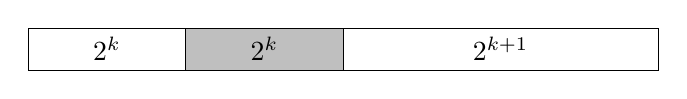
\begin{tikzpicture}[every node/.style={draw},
      small/.style={minimum width=2cm},
      large/.style={minimum width=4cm}]]
      \node[small] (m0) {$2^k$};
      \node[small,fill=gray!50] (m1) [right of=m0,xshift=1cm] {$2^k$};
      \node[large] (m2) [right of=m1,xshift=2cm] {$2^{k+1}$};
    \end{tikzpicture}
  \end{center}
  
  \reinitrand[counter=rand,first=3,last=5]
  A memória total disponível é $2^m$ unidades de memória. Se o valor de
  $k$ for igual a $\R$, responda às seguintes questões:
  
\begin{parts}
  \part Qual o valor de $m$?
  \part Qual a quantidade de memória que está ocupada em unidades de memória?
  \part Qual a quantidade de memória livre?
  \part Qual a quantidade total de memória?
\end{parts}
}

\def\PAGING{ 
  \question[3]~Dois processos possuem as seguintes
  páginas lógicas: $P1 = \{a, b, c\}, P2 = \{1, 2, 3, 4\}$. Supondo
  que o sistema operacional disp\~oe de 4 páginas físicas para alocar
  as páginas lógicas, fa\c{c}a um esboço gráfico para a ocupação das
  páginas lógicas que forem requisitadas na seguinte sequência:

  \reinitrand[counter=rand,first=1,last=4]
  \begin{center}
    $\{b,a,\R,\R,\R,\R,\R,\R,b,\R,a,\R,\R,\R,a,b,c\}$
  \end{center}
  utilizando os seguintes algoritmos de substituição de páginas:\\
 
  \begin{parts}
  %\part FIFO;
    \part Relógio;
    \part Segunda chance;
    \part LRU.
  \end{parts}\smallskip

  Calcule a taxa de falta de páginas (porcentagem de {\em page fault})
  para os algoritmos.

  \question[0,5] A tabela de páginas armazena informa\c{c}\~oes a
  respeito do mapeamento entre os endere\c{c}os l\'gicos e f\'isicos
  de mem\'oria. H\'a um campo de tamanho de 1 bit que informa se a
  p\'agina est\'a na mem\'oria f\'isica ou disco r\'igido e outro
  campo que marca se houve altera\c{c}\~ao no conte\'udo da p\'agina
  na mem\'oria f\'isica para que esta seja gravada em disco antes de
  ser retirada da tabela. Os bits que representam estes campos s\~ao
  chamados respectivamente de:

\begin{enumerate}[(a)]
{\item refer\^encia e sujeira.}
{\item validade e refer\^encia.}
{\item sujeira e validade.}
{\item validade e sujeira.}
{\item sujeira e refer\^encia.}
\end{enumerate}

\question[0,5] A tabela de p\'aginas localiza-se no (a):

\begin{enumerate}[(a)]
{\item Mem\'oria cache.}
{\item Registrador.}
{\item Disco Rígido.}
{\item Mem\'oria principal (DRAM).}
{\item Mem\'oria ROM.}
\end{enumerate}

}

\ifnum1=2
O que \'e a troca de mem\'oria ({\em swapping}) do espa\c{c}o de endere\c{c}amento de
processos?


\paragraph{Quest\~ao 6. (1,5 ponto)}
Defina as 4 entidades b\'asicas dos sistemas de
arquivos.

\paragraph{Quest\~ao \ex{}. (1,5 ponto)}
Defina e d\^e exemplos das classes gen\'ericas de dispositivos de entrada
e sa\'ida.

\fi